\chapter{Introduction}
%The main goal of this thesis is to develop a model that can solve geometric problems. The goal is to solve problems presented in the construction game Euclidea.
\section{Goal}
The goal of this thesis is to create a solver for geometric construction problems. The solver may use only a ruler, compass and tools representing a sequence of ruler and compass usages, such as the Perpendicular Bisector tool or the Parallel tool. The goal is to develop a machine learning model based on a convolutional neural network that will be able to predict the next step of the construction. Input for this model is an image of the scene containing the initial state and the goal. Outputs of this model are masks and bounding boxes of detected objects. Those masks have to be processed into actions representing construction steps. We can see examples of inputs and outputs in Table \ref{Zeta06_example}. This model should be able to solve as many geometric construction problems as possible. Furthermore, the model should also be able to solve problems for which it was not trained. Finally, the goal is to test the model accuracy on the problems that were both seen and unseen during the training. To test and train our model, we use geometric problems from Euclidea, which is an online construction game.

\begin{longtable}{p{7.25cm}p{7.25cm}}

\subfloat{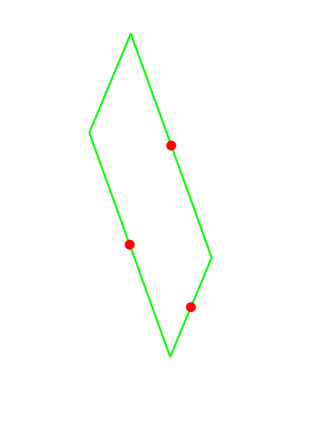
\includegraphics[scale=0.4]{img/Zeta-06_example/input_image0.png}} &
\subfloat{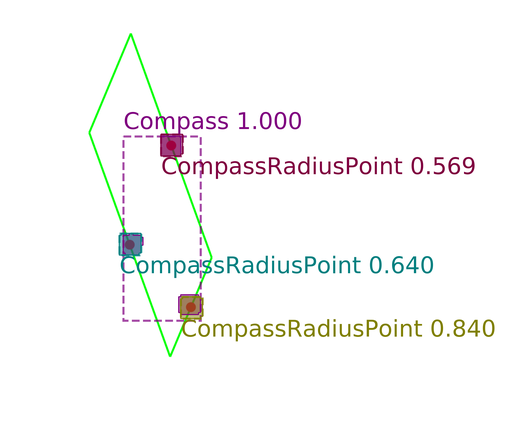
\includegraphics[scale=0.4]{img/Zeta-06_example/output_image0.png}}\\

\begin{small}a) Level definition: Construct a parallelogram given three of the midpoints. The green color denotes the goal and the red denotes the current state of the construction.\end{small}
& 
\begin{small}
b) Prediction of the Mask {R-CNN} model for step 1. In the figure, we can see a prediction of the Compass tool. Each detection has a bounding box highlighted with a dashed rectangle and mask, which is filled with the same color as the corresponding bounding box. Note that the Compass tool should have two radius points and one center point but there is missing detection of the center point. In this situation can be any radius point used as the center point. Hence it is randomly chosen. The green color denotes the goal and the red denotes the current state of the construction. \end{small}
\\
 

\subfloat{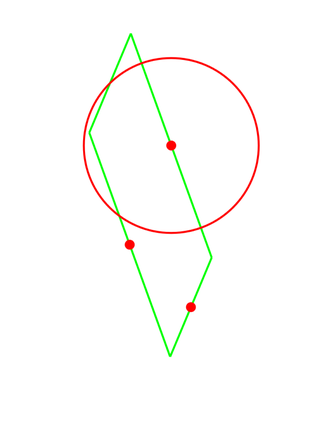
\includegraphics[scale=0.4]{img/Zeta-06_example/input_image1.png}} &
\subfloat{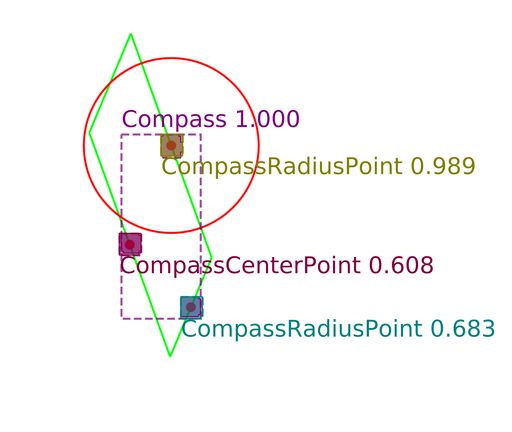
\includegraphics[scale=0.4]{img/Zeta-06_example/output_image1.png}}\\
\begin{small}
c) Step 1. In the figure, we can see that the Compass tool created a circle. \end{small}
&
\begin{small}d) Prediction for step 2. We can see another detection of the Compass tool. However, the difference is that the circle center is now specified. \end{small}\\

\subfloat{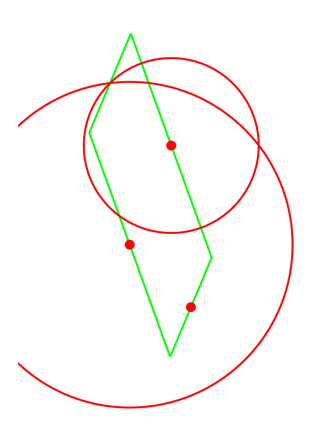
\includegraphics[scale=0.4]{img/Zeta-06_example/input_image2.png}} &
\subfloat{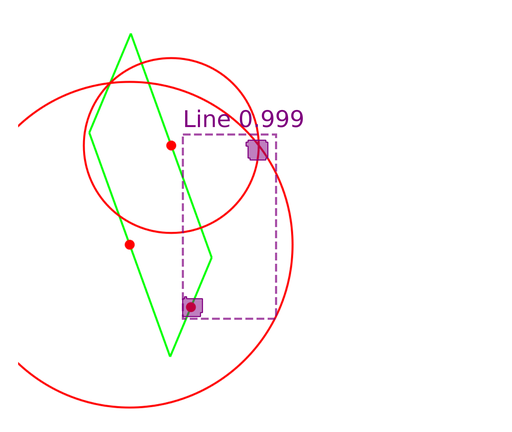
\includegraphics[scale=0.4  ]{img/Zeta-06_example/output_image2.png}}\\
\begin{small}
e) Step 2. \end{small}& 
\begin{small}f) Prediction for step 3. Based on this prediction a line will be constructed.\end{small}\\

\subfloat{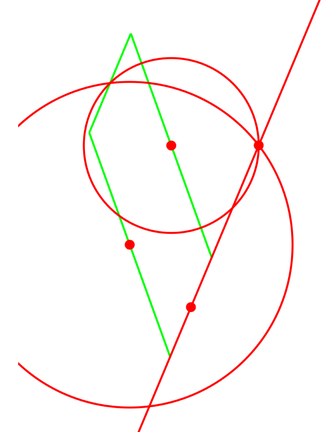
\includegraphics[scale=0.4  ]{img/Zeta-06_example/input_image3.png}} &
\subfloat{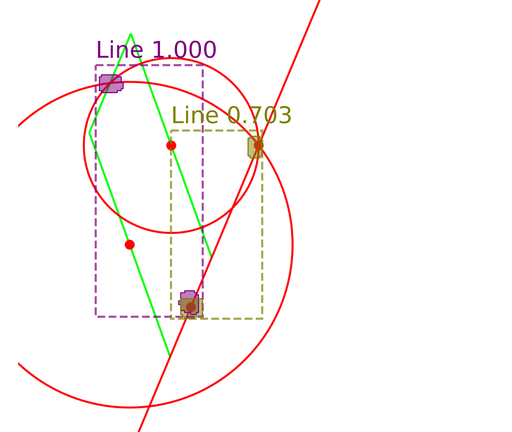
\includegraphics[scale=0.4  ]{img/Zeta-06_example/output_image3.png}}\\
\begin{small}
g) Step 3. The last line constructed part of the goal, one side of the parallelogram. \end{small}
& 
\begin{small}h) Prediction for step 4. Based on this prediction, a line will be constructed. Note that there are two line tool predictions. However, one of these prediction has a significantly lower Mask {R-CNN} score. \end{small}\\

\subfloat{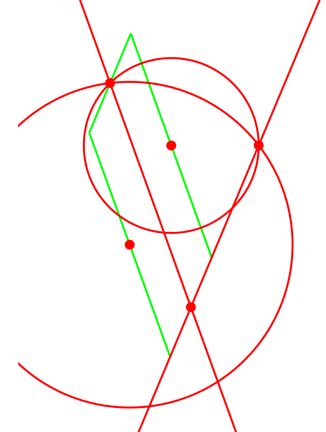
\includegraphics[scale=0.4  ]{img/Zeta-06_example/input_image4.png}} &
\subfloat{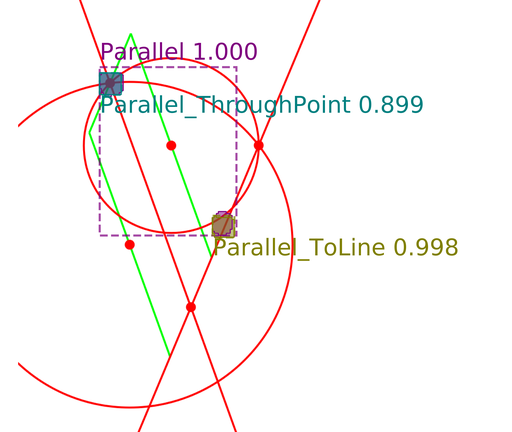
\includegraphics[scale=0.4  ]{img/Zeta-06_example/output_image4.png}}\\
\begin{small}
i) Step 4.\end{small} & \begin{small} j) Prediction for step 5. Based on this prediction a parallel line will be constructed.\end{small}\\

\subfloat{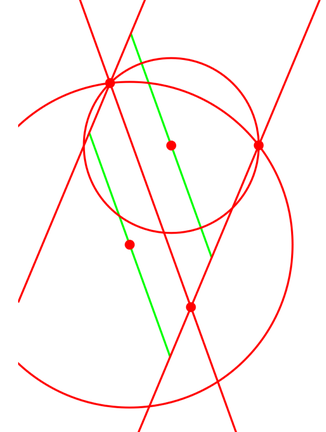
\includegraphics[scale=0.4  ]{img/Zeta-06_example/input_image5.png}} &
\subfloat{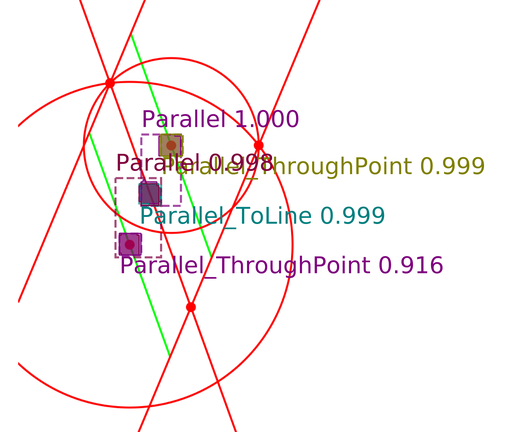
\includegraphics[scale=0.4  ]{img/Zeta-06_example/output_image5.png}}\\
\begin{small}
k) Step 5. The last parallel line constructed part of the goal, another side of the parallelogram.\end{small}&\begin{small}l) Prediction for step 6. Based on this prediction, a parallel line will be constructed. Note that there are two predictions of the parallel tool. Both of these parallels have to be constructed in order to finish the goal. In this step, detection with a higher Mask {R-CNN} score will be constructed.\end{small}\\

\subfloat{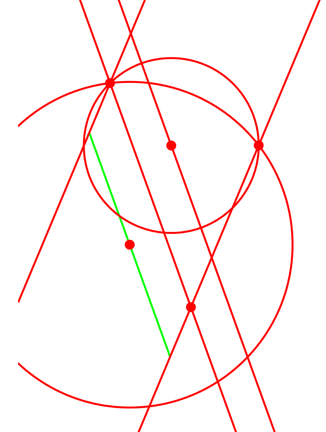
\includegraphics[scale=0.4  ]{img/Zeta-06_example/input_image6.png}} &
\subfloat{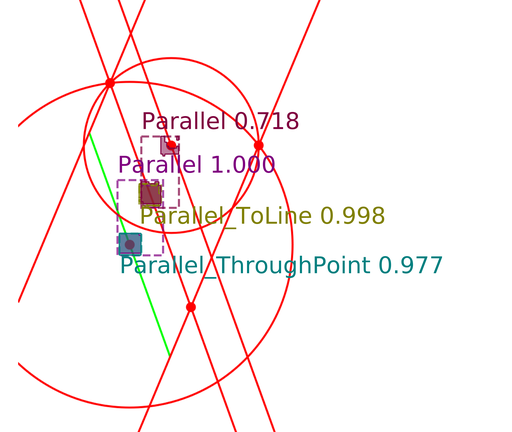
\includegraphics[scale=0.4  ]{img/Zeta-06_example/output_image6.png}}\\
\begin{small}
m) Step 6. The last parallel line constructed another part of the goal, one side of the parallelogram. \end{small}&\begin{small} n) Prediction for step 7. Based on this prediction, a parallel line will be constructed. Both predictions are still present. However, the prediction used in the previous step has a lower Mask {R-CNN} score. Hence, it is not used now.\end{small}\\

\subfloat{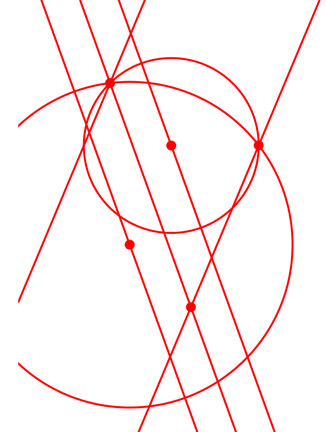
\includegraphics[scale=0.4  ]{img/Zeta-06_example/input_image7.png}}\\
\begin{small}
o) step 7. The last parallel line constructed the last part of the goal. Hence the geometric problem is successfully constructed.\end{small}\\

\caption{Example construction of level \textit{Zeta-12}: Parallelogram by 3 midpoints. The table contains 7 steps of the construction. Each step contains current progress on the left and Mask {R-CNN} prediction for a new step on the right. The green color denotes the goal and the red denotes the current state of the construction. Other colors mark prediction masks, bounding boxes, classes and scores for each detected object.}
\label{Zeta06_example}
\end{longtable}



\section{Motivation}
% - most existing work solve geometric constructions from known analytical models of individual primitives. The first motivation for this work is answering the question whether  whether geometric constructions can be solved given only the image input. 
% - this is similar to humans, which can ...

% - We wil show that the learnet recognizer is to some extent transferrable across different constructions and hence it opens up the possibility of using similar models hypothesis generators for automatic geometric theorem proovers [].

% - This project is a step towards developing methods that combine machine learning with machine reasoning over noisy visual (or visual and text [Seo15]) inputs. The long-term goal is developing automatic “virtual AI assistants” that can help mathematicians with complex proofs [Hales17] or reason about text and associated illustrations (e.g. automatic patent lawyer assistant). 
The first motivation for this work is to answer whether geometric constructions can be solved given only the image input. Most existing methods solve geometric constructions with knowledge of the analytical equitations behind each geometric primitive in the geometric problem.
\newline \newline
The second motivation is to develop a method that can solve geometric construction problems similar to how humans solve these problems. Since humans are capable of solving geometric problems without knowledge of the analytical model, moreover, we might have only a sketch that is an approximation of a geometrical problem. In this situation, we are forced to use only image data about the problem.
\newline \newline
The third motivation is a step towards developing an automatic geometric theorem prover. We will show that our learned recognizer is, to some extent, transferable across different constructions, and hence it opens up the possibility of using similar models hypothesis generators. This hypothesis generator can be used as an assistant for a human solver or a possible reinforcement learning method that will learn to combine proposed hypotheses.

%In some situations, we do not have an exact analytical model behind the scene. We might have only a sketch that is an approximation of a real-life problem. Furthermore, real-life problems cannot be precisely measured, and there is always some measurement error.  Input for our method is only an image of the scene with a highlighted goal. Our method's output is then a sequence of instructions on using the ruler and compass to construct the given problem. Our method's advantage is also that it provides hypotheses of construction steps, which might serve as an assistant for a human solver. Furthermore, the method's hypotheses proposal is generated with one forward pass through the neural network based on Mask {R-CNN}. Thus hypotheses are generated within a minute on a standard computer.
\section{Why is it difficult?}
In the course of the thesis we have to deal with four major problems: problem variability, construction ambiguity, object detection and training data generation. Figure \ref{variabilty_problem} is an illustration of the problem variability. The same geometric problem can have different variants, e.g.~different scale, rotation or different position of individual geometric primitives. Furthermore, each problem can be solved in an infinite number of ways. The most straightforward way to solve these problems is an exhaustive search of the construction space. The majority of existing methods use an analytical model to generate the next steps quickly. However, even with smart heuristics, a complete search of more complex problems can take up to days or even months of searching. Nevertheless, our goal is to play construction game Euclidea, so we aim to have a reasonable reaction time, but exhaustive search is often too slow.
\newline \newline
On top of that, we have to deal with object detection because only data about the geometric problem our method receives as input is an image. To recognize individual geometric primitives and their relative positions, part of our approach is object detection architecture. However, object detection architecture, such as Mask {R-CNN}, requires large amount of annotated data and computing time to be properly trained. Furthermore, training data have to be constructions that can be solved based on the image data. To train a model that can solve a geometric problem, we have to generate training data, which are constructions of multiple different configurations of the given problem. While creating new configurations of a problem, we have to create well-defined variants that are solvable. Problem variability, detection and data generation can be challenging apart, but we have to deal with them at once.
\begin{figure}[h!]
\begin{tabular}{cccc}
     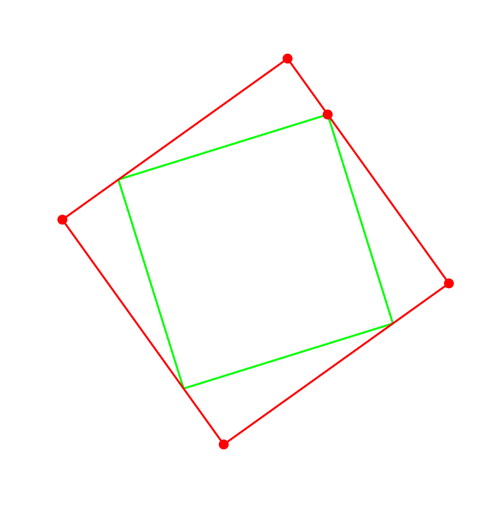
\includegraphics[width=0.2\textwidth]{img/problem_variability/problem_variability_1.png}
     &
     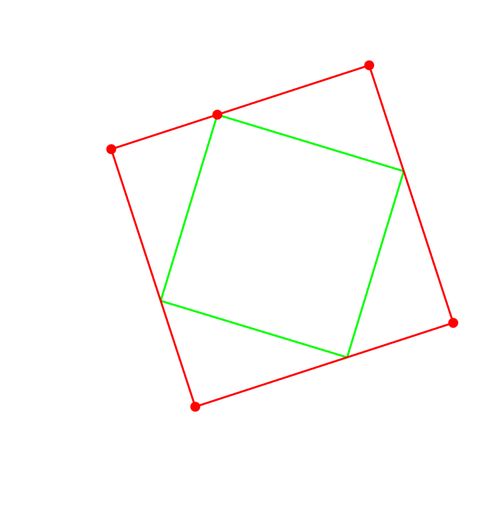
\includegraphics[width=0.2\textwidth]{img/problem_variability/problem_variability_2.png}&
     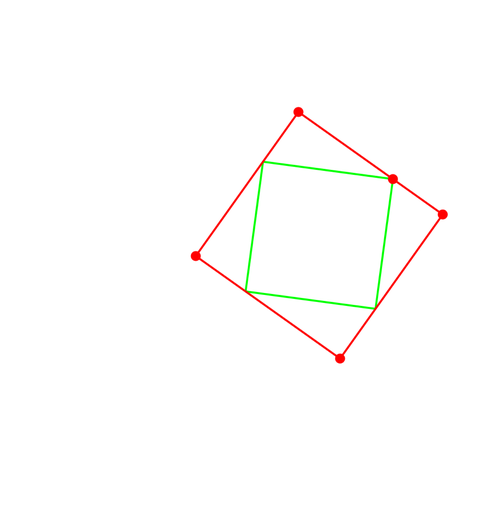
\includegraphics[width=0.2\textwidth]{img/problem_variability/problem_variability_3.png}
     &
     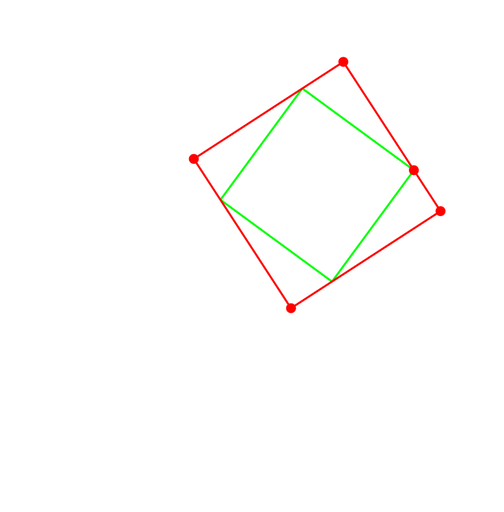
\includegraphics[width=0.2\textwidth]{img/problem_variability/problem_variability_4.png}
     \\
     a)  & b) & c) & d)
     \\
     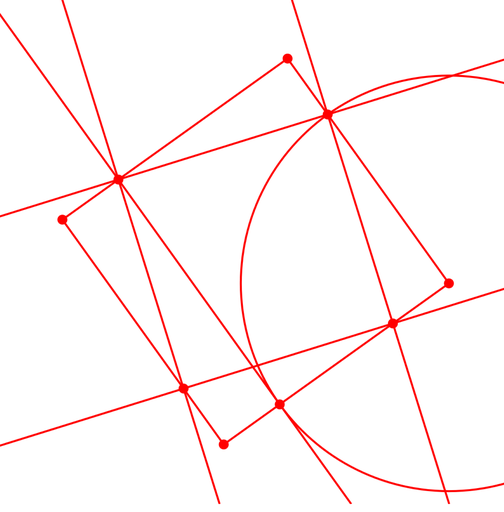
\includegraphics[width=0.2\textwidth]{img/problem_variability/problem_variability_1_solved.png}
     &
     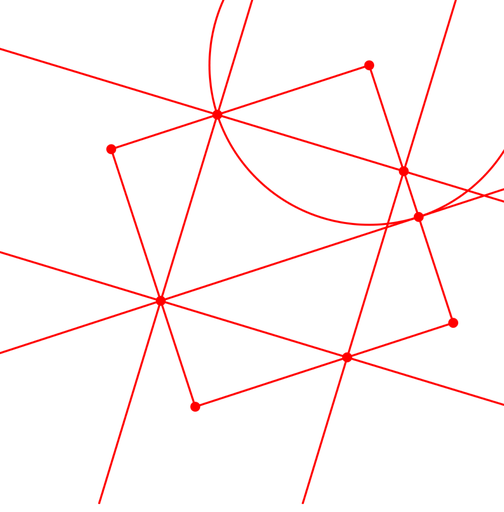
\includegraphics[width=0.2\textwidth]{img/problem_variability/problem_variability_2_solved.png}
     &
     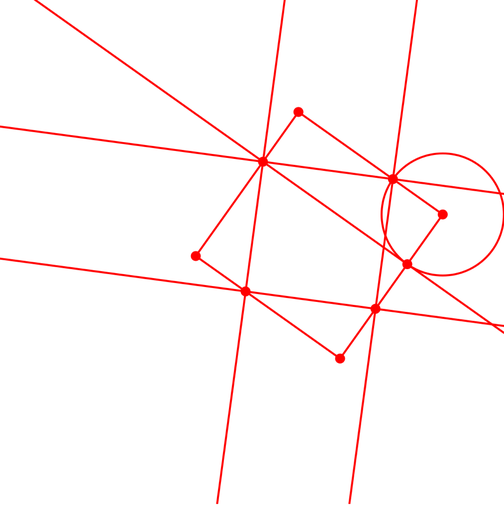
\includegraphics[width=0.2\textwidth]{img/problem_variability/problem_variability_3_solved.png}
     &
     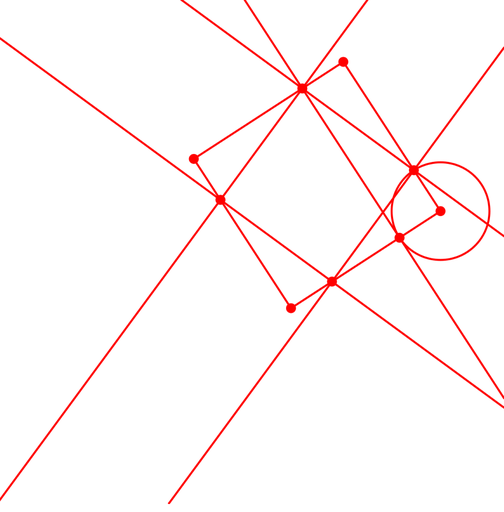
\includegraphics[width=0.2\textwidth]{img/problem_variability/problem_variability_4_solved.png}
     \\
     1) & 2) & 3) & 4)
     \\
\end{tabular}
\caption{Four instances of the same geometric problem, inscribe a square in the square when a vertex is given. Each instance contains a problem definition and a solution. In the top row are definitions of the problem and in the bottom row are corresponding solutions. Figures contains current states (red) d remaining goals (green).}
\label{variabilty_problem}
\end{figure}

\section{Related work}
Most geometric construction solvers utilize the analytical model for solving the problems. In our setup, we aim to find a solution to problems that we know are solvable. However, the focus of the research is also to prove or disprove the existence of a solution to a given problem. This proving process is also known as automated theorem proving (ATP). Methods of proving can be an exhaustive search for a solution \cite{ancient_problem}, by deriving new facts based on well-know properties in the problem or a combination of both \cite{botana15}. ATPs can also be solved with resolution theorem provers
and a coherent logic theorem provers \cite{stojanovicdurdevic:hal-01091011}. Alternatively, there are ATPs that can answer SAT-questions about geometric problems \cite{seo15}. For example, a question like: Based on known facts, are given lines perpendicular or not? On the other hand, some complex problems, such as Kepler conjecture, require assistance from ATP to be properly proven \cite{DBLP:journals/corr/abs-1211-7012} \cite{hales17}.
\newline 
In this thesis we combine ATP with an object detection architecture. One of the well-known architectures is the Mask {R-CNN} \cite{DBLP:journals/corr/HeGDG17}, which detects mask and bounding boxes in images and videos. This architecture is also used for pose estimation \cite{DBLP:journals/corr/abs-1712-09184}, \cite{Girdhar_2019_CVPR} or to estimate 3D motion and forces \cite{DBLP:journals/corr/abs-1904-02683}.

\section{Outline}
In Chapter \ref{euclidea_chapter}, we describe our implementation of Euclidea, an online construction game with an interface matching the desired agent. This chapter also describes how to generate new configurations of geometric problems used as training data for supervised learning. Then in Chapter \ref{chapter_exhaustive_search}, we analyze the difficulty of the problem by estimating the branching factor of the exhaustive tree search. In Chapter \ref{mrcnn_chapter}, we introduce a new approach based on Mask {R-CNN} as our primary model for supervised learning approach for the geometric construction problems. Then in Chapter \ref{chapter_unseen_levels}, we analyze the performance of Mask {R-CNN} models on the problems that were not seen during the training. To do so, we also describe the hypothesis tree search to search hypotheses obtained from multiple Mask {R-CNN} models. In the last Chapter \ref{experiment_chapter},
we describe multiple components of this model and experimentally demonstrate their benefits. Then we analyze the results of our best model on levels seen during the training. Then we analyze the accuracy of models for each level pack on unseen geometric problems with leave-one-out evaluation. Finally, we present multiple example solutions of Euclidea geometric problems.

